\documentclass[journal,hidelinks]{IEEEtran}
\usepackage[utf8]{inputenc}
\usepackage[
  pdftitle={Final Exam},
  pdfauthor={Andrei Purcarus},
  pdfsubject={ECSE-534 -- Analog Microelectronics}
]{hyperref}
\usepackage{graphicx}
\usepackage[all]{hypcap}
\usepackage{cleveref}
\usepackage{indentfirst}
\usepackage[per-mode=symbol]{siunitx}
\usepackage{amsmath}

\title{ECSE-534 \\ Analog Microelectronics \\ Final Exam}
\author{Andrei~Purcarus,~260631911,~\IEEEmembership{McGill~University} \\ \href{mailto:andrei.purcaruscraciun@mail.mcgill.ca}{andrei.purcaruscraciun@mail.mcgill.ca}}

\begin{document}
\sloppy

\maketitle

\section{Introduction}

\IEEEPARstart{T}{his} report follows the design, simulation, and analysis of an anti-aliasing filter for a $\Delta \Sigma$ data converter using a 0.13 micron process from IBM. We used Cadence to simulate the design in said process. The filter was required to adhere to the topology shown in \Cref{fig:filter_topology} and meet the following specifications:
\begin{itemize}
  \item A DC gain of $\SI{1}{\volt\per\volt}$.
  \item A passband from DC to $\SI{100}{\kilo\hertz}$.
  \item A maximum attenuation of $\SI{0.1}{\deci\bel}$ in the passband.
  \item A maximum phase shift of $\SI{10}{\degree}$ in the passband.
  \item A minimum attenuation of $\SI{40}{\deci\bel}$ at frequencies over $\SI{15}{\mega\hertz}$.
  \item An input resistance of at least $\SI{1}{\kilo\ohm}$.
  \item An output resistance of at most $\SI{20}{\ohm}$.
  \item An output voltage swing of $\SI{0.9}{\volt}$ around an analog ground level of $\SI{0.6}{\volt}$.
  \item A maximum RMS noise level of $\SI{100}{\micro\volt}$.
\end{itemize}

The filter must meet these specifications while driving a $\SI{1}{\pico\farad}$ load capacitance that represents the input capacitance of the $\Delta \Sigma$ data converter.

\begin{figure}[!htb]
  \centering
  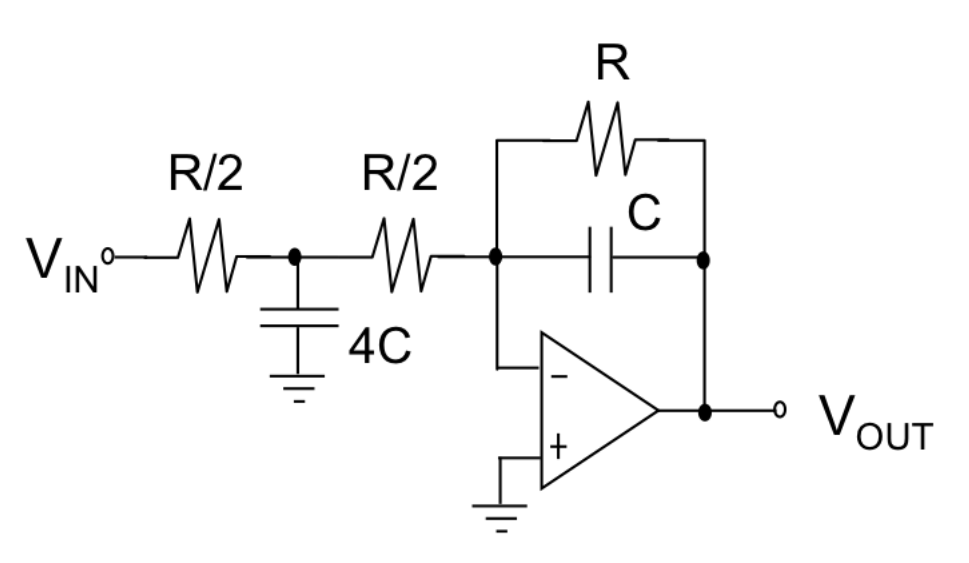
\includegraphics[width=\columnwidth]{schematics/filter_topology.png}
  \caption{A schematic of the second-order anti-aliasing filter topology.}
  \label{fig:filter_topology}
\end{figure}

To meet these requirements, we first calculated the required values for the passive components of the filter. Then, we modified the operational amplifier we designed in the past assignments to meet the specifications. Next, we assembled the filter and verified that it meets the requirements. Finally, we discussed a rough sketch of the layout of the filter.

\begin{figure*}[!htb]
  \centering
  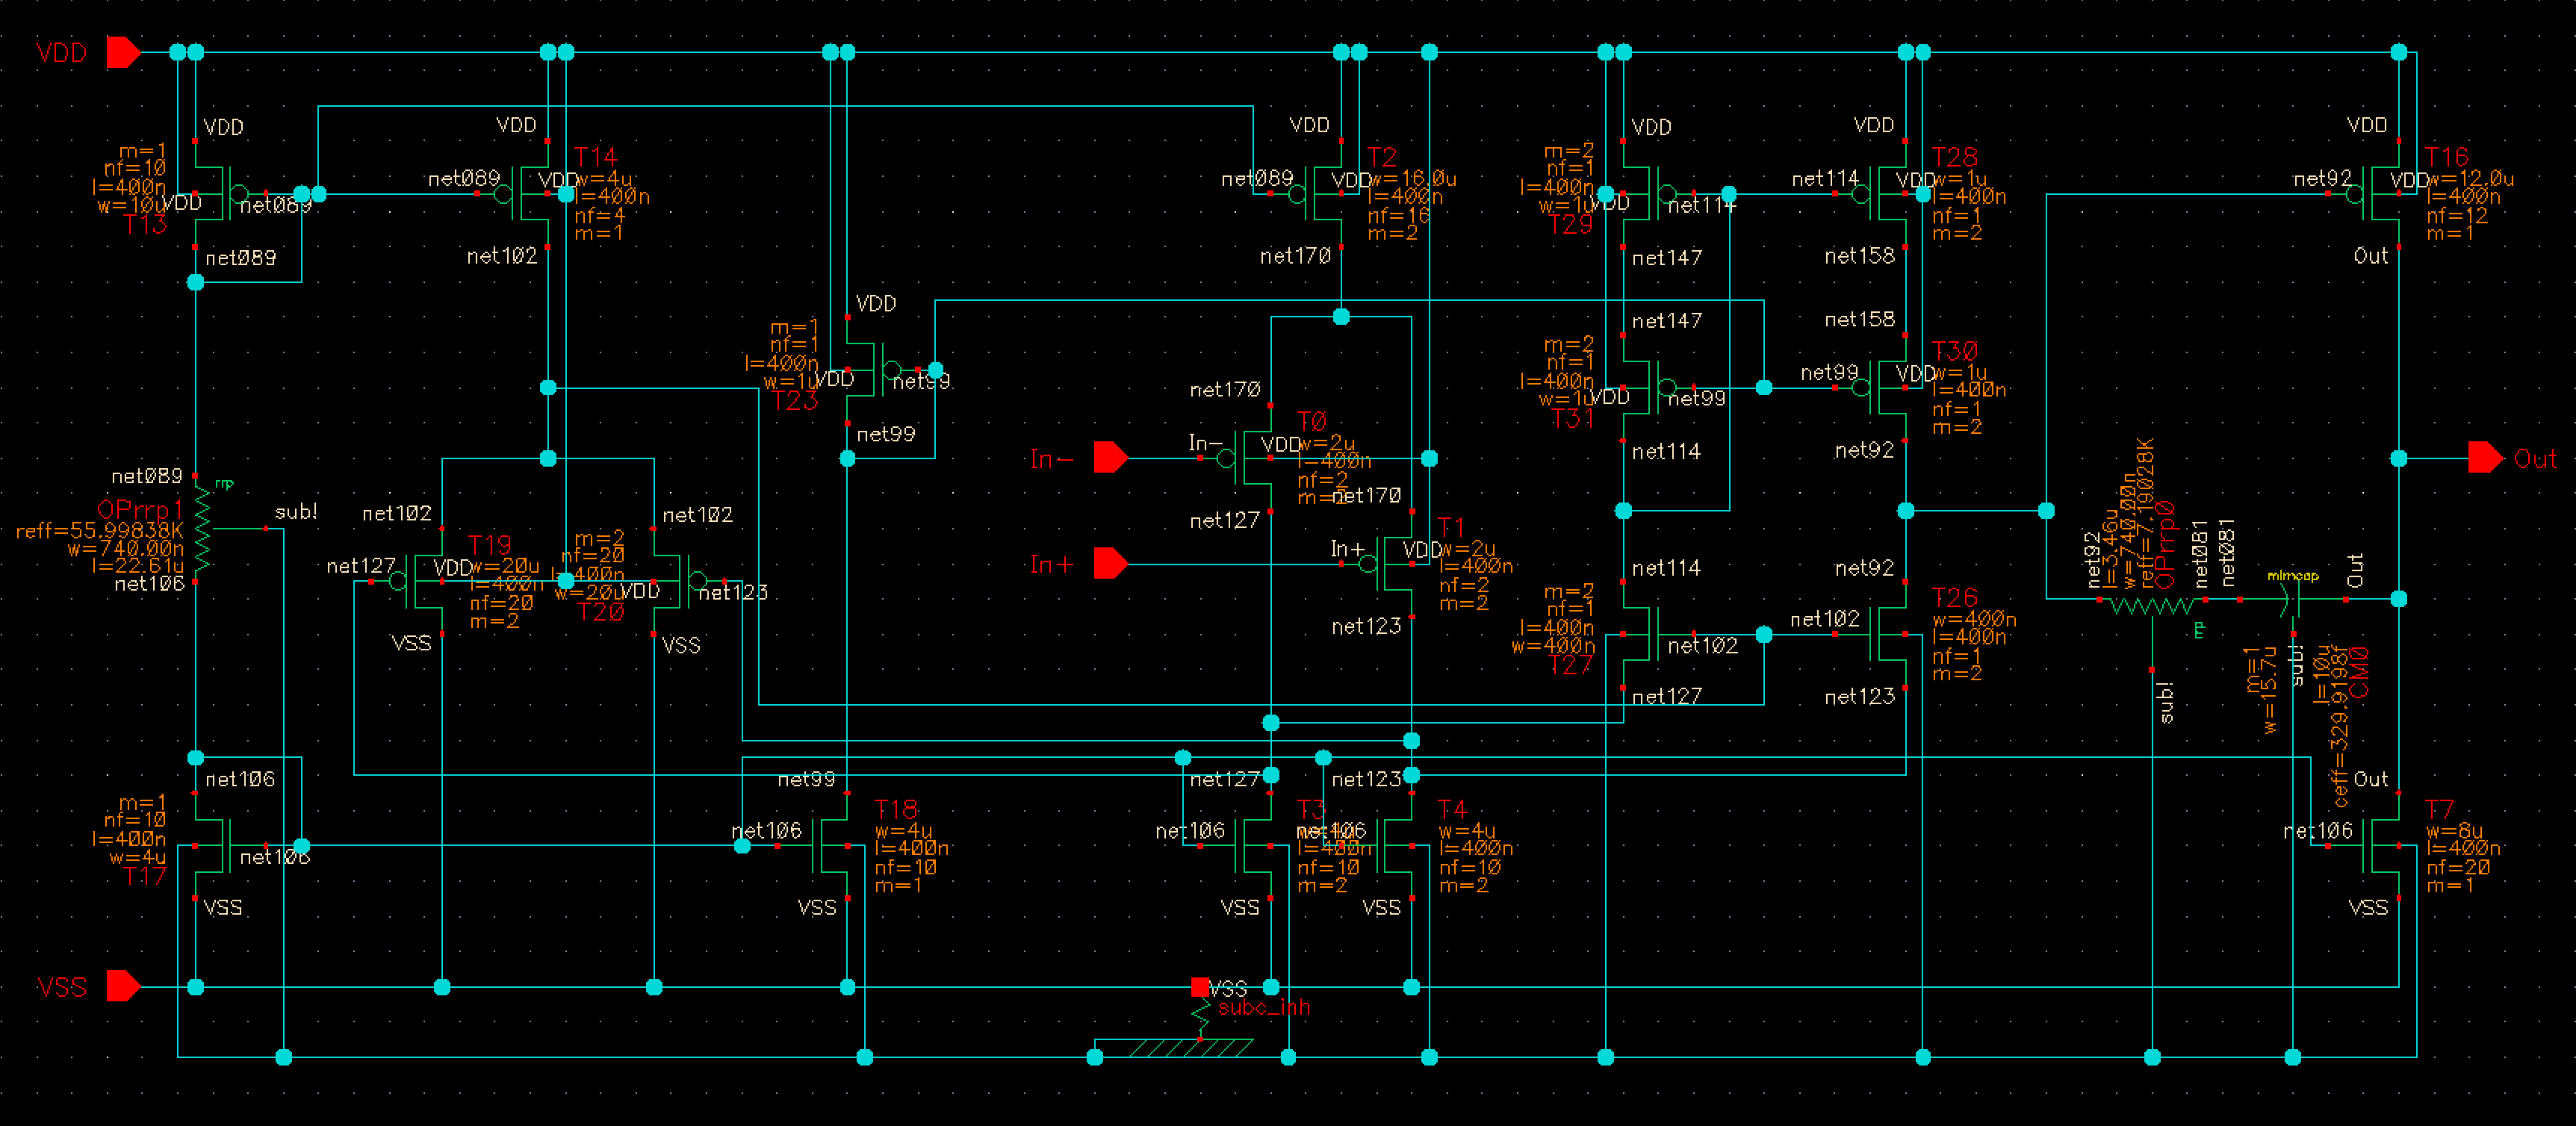
\includegraphics[width=\textwidth]{schematics/folded_cascode.png}
  \caption{A schematic of the operational amplifier designed in past assignments.}
  \label{fig:folded_cascode}
\end{figure*}

\begin{figure*}[!htb]
  \centering
  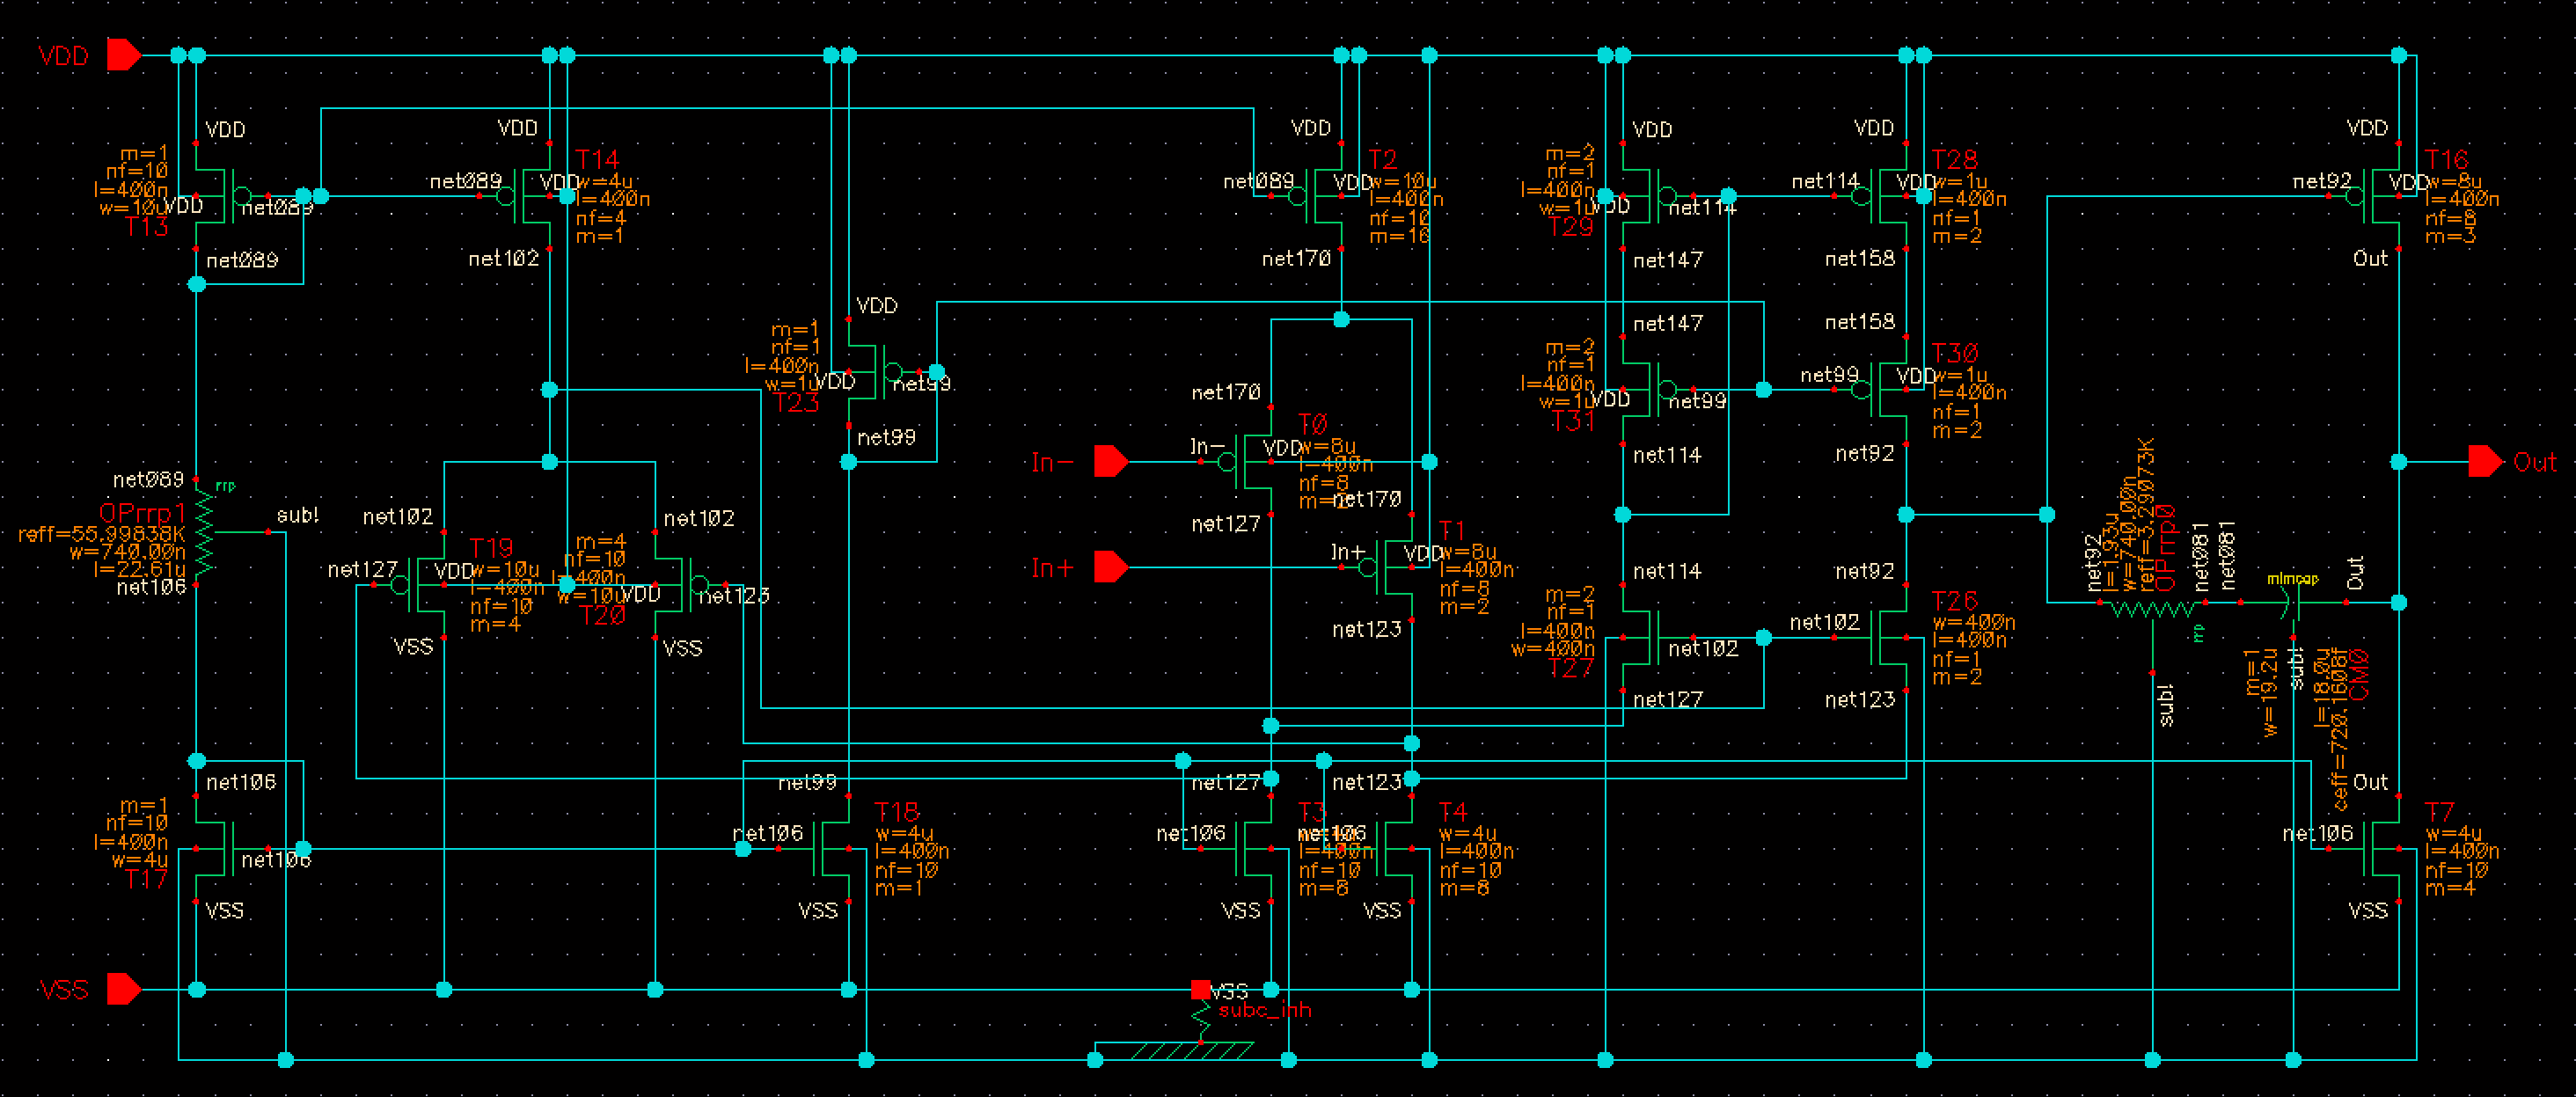
\includegraphics[width=\textwidth]{schematics/folded_cascode_2.png}
  \caption{A schematic of the modified operational amplifier made to meet the requirements.}
  \label{fig:folded_cascode_2}
\end{figure*}

\begin{figure*}[!htb]
  \centering
  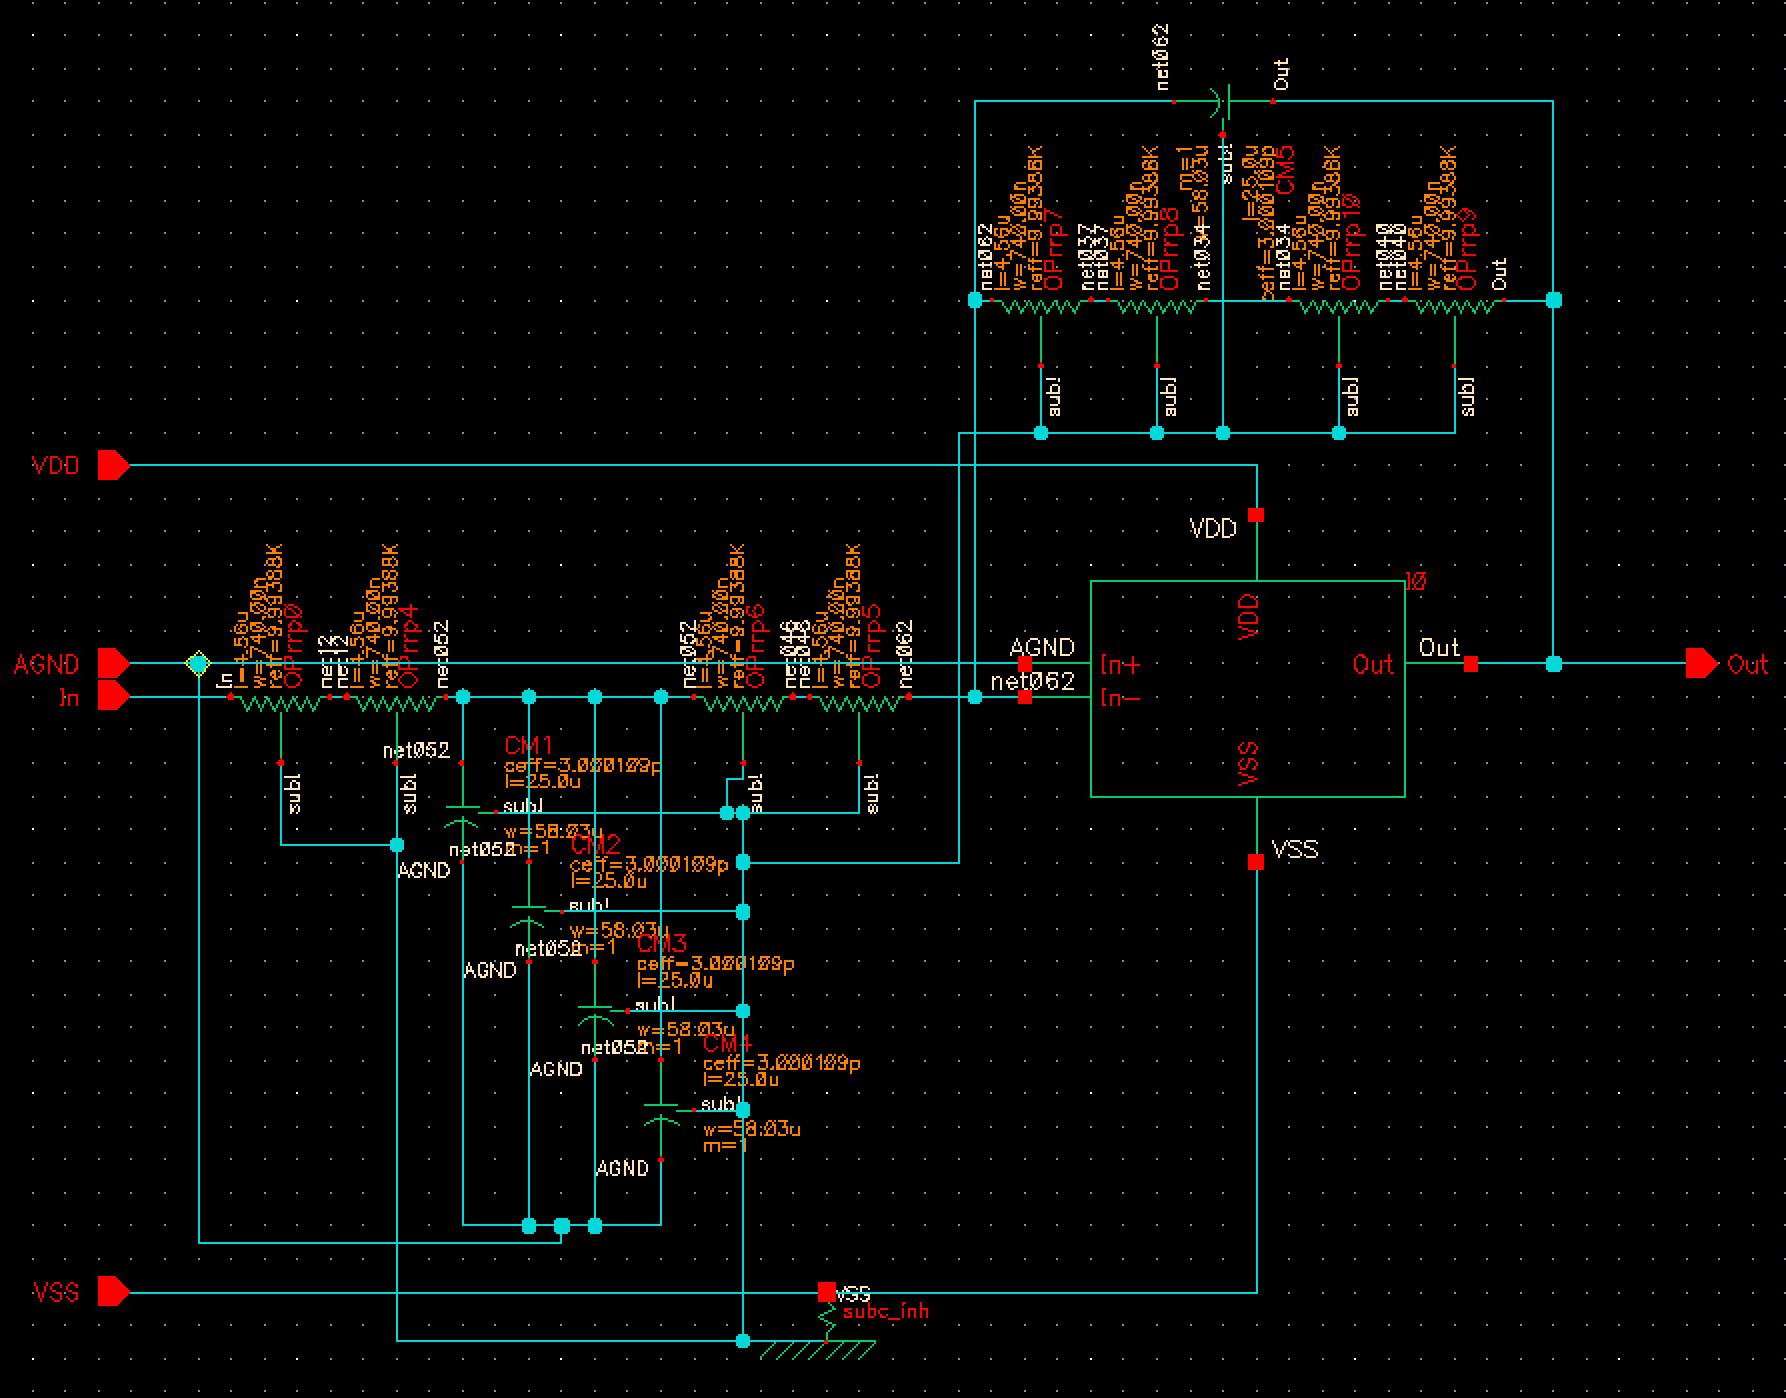
\includegraphics[width=\textwidth]{schematics/filter.png}
  \caption{A schematic of the anti-aliasing filter.}
  \label{fig:filter}
\end{figure*}

\section{Filter Design}

We first translated the given specifications into restrictions on our circuit. We started by deriving the transfer function of the filter as
\begin{align}
H(s) &= \frac{-R}{1 + s R C} \frac{1}{R/2} \frac{1/2}{1 + s R C} \\
     &= \frac{-1}{(1 + s R C)^2}
\end{align}
This result tells us that the DC gain is $-1$ and the bandwidth is given by $f_{3dB} = 1 / 2 \pi R C$.

In order to gain more insight into the operation of the filter, we added a relative mismatch $\Delta$ to the components in the feedback network. We thus obtained
\begin{align}
H(s) &= \frac{-R (1 + \Delta_R)}{1 + s R C (1 + \Delta_R) (1 + \Delta_C)} \frac{1}{R/2} \frac{1/2}{1 + s R C} \\
     &\approx \frac{-R (1 + \Delta_R)}{1 + s R C (1 + \Delta_R + \Delta_C)} \frac{1}{R/2} \frac{1/2}{1 + s R C}
\end{align}
This result tells us that the DC gain can be approximated as $-(1 + \Delta_R)$ and that there are two poles formed, one at $f_1 = 1 / 2 \pi R C$ and the other at $f_2 = 1 / 2 \pi R C (1 + \Delta_R + \Delta_C)$.

The given DC gain requirement means that the feedback resistors in the circuit must match well. In addition, the DC gain of the operational amplifier must be high, say at least $\SI{60}{\deci\bel}$.

The given attenuation requirements mean that we must have $f_{3dB} \gg \SI{100}{\kilo\hertz}$ and $f_{3db} \ll \SI{15}{\mega\hertz}$. Since a second order filter has a roll-off of about $\SI{40}{\deci\bel}$ per decade, this translates approximately to $f_{3db} < \SI{1.5}{\mega\hertz}$.

The given input resistance requirement means that $R > \SI{1}{\kilo\hertz}$. The given output resistance requirement means that we must have $2 R_{out} < \SI{20}{\ohm}$ for the operational amplifier, where $R_{out}$ is the output resistance of the amplifier in the unity gain configuration.

The given voltage swing requirements translate directly into equivalent requirements for the operational amplifier.

The given noise requirement must be separated between two sources: the thermal noise generated by the feedback network and the noise generated by the amplifier. We therefore allocate an RMS noise budget of $\SI{50}{\micro\volt}$ to each.

The RMS thermal noise generated by the feedback network can be approximated as
\begin{align}
v_{n,rms} = \sqrt{\frac{kT}{C} + \frac{kT}{4C}}
\end{align}
Therefore, we have
\begin{align}
v_{n,rms} &< \SI{50}{\micro\volt} \\
\sqrt{\frac{kT}{C} + \frac{kT}{4C}} &< \SI{50}{\micro\volt} \\
C &> \SI{2}{\pico\farad}
\end{align}

The noise generated by the amplifier is harder to quantify. However, since the feedback gain of our circuit is $1 / 2$, the output spectral noise density of the amplifier in this circuit will be equivalent to the input-referred spectral noise density measured in open loop simulation times $2$. Thus, we require an input-referred RMS noise level of at most $\SI{50}{\micro\volt} / \sqrt{2} = \SI{35}{\micro\volt}$.

Therefore, the requirements for the feedback network are
\begin{equation}
R > \SI{1}{\kilo\ohm}
\end{equation}
\begin{equation}
C > \SI{2}{\pico\farad}
\end{equation}
\begin{equation}
\SI{100}{\kilo\hertz} \ll \frac{1}{2 \pi R C} < \SI{1.5}{\mega\hertz}
\end{equation}

To minimize the size of the capacitors used, we chose to use $C = \SI{3}{\pico\farad}$. Then, to allow for at least a $\SI{20}{\percent}$ margin on the upper bandwidth, we chose to use $f_{3dB} = \SI{1}{\mega\hertz}$, and thus $R = \SI{53}{\kilo\ohm}$.

\section{Operational Amplifier Design}

From the previous section, the main requirements for the operational amplifier are a DC gain of at least $\SI{60}{\deci\bel}$, a maximum output resistance of $\SI{10}{\ohm}$ in the unity gain configuration, and an input-referred RMS noise level of at most $\SI{35}{\micro\volt}$ over the given bandwidth. In addition, we require that the unity gain frequency of the amplifier should be at least 10 times our chosen filter bandwidth, at $\SI{10}{\mega\hertz}$.

To meet these specifications, we reused the operational amplifier designed in the past assignments. A schematic is shown in \Cref{fig:folded_cascode}. This amplifier has a DC gain of $\SI{73}{\deci\bel}$, a unity gain bandwidth of $\SI{40}{\mega\hertz}$, an output resistance in the unity gain configuration of $\SI{12.9}{\ohm}$, and a total input-referred RMS noise of $\SI{65}{\micro\volt}$ between $\SI{1}{\hertz}$ and $\SI{100}{\kilo\hertz}$.

These results show that the amplifier does not meet the specifications for noise and output resistance. In order to modify the amplifier to meet the specifications, we performed a series of transformations on our initial circuit.

A noise analysis in Cadence indicated that the main contributors to the noise level were transistors $T_0$, $T_1$, $T_3$, and $T_4$, with a total contribution of $\SI{92.68}{\percent}$. Since flicker noise is inversely proportional to transistor area, we needed to scale the widths of these transistors upward. We achieved this by scaling the widths of $T_0$, $T_1$, $T_3$, and $T_4$ by a factor of $4$, and then scaling the width of $T_2$ to provide sufficient current to $T_0$ and $T_1$ to avoid disturbing the operating point of the other transistors in the circuit. This transistor ended up being scaled by a factor of $5$.
In addition, to meet the output resistance specification, we needed to scale the current in the output branch upward. We achieved this by scaling the widths of both $T_7$ and $T_{16}$ by a factor of $2$.
This also had the effect of scaling our bandwidth upward, so we scaled $C_c$ to $\SI{0.72}{\pico\farad}$ and $R_c$ to $\SI{3.3}{\kilo\ohm}$ to compensate.
The resulting amplifier is shown in \Cref{fig:folded_cascode_2}.

We then measured the amplifier's characteristics to confirm that it now met the specifications. The amplifier now had a DC gain of $\SI{77}{\deci\bel}$, a unity gain bandwidth of $\SI{53}{\mega\hertz}$, an output resistance in the unity gain configuration of $\SI{4.1}{\ohm}$, and a total input-referred RMS noise of $\SI{32}{\micro\volt}$ between $\SI{1}{\hertz}$ and $\SI{100}{\kilo\hertz}$. The first two poles were also moved to $\SI{8}{\kilo\hertz}$ and $\SI{102}{\mega\hertz}$, and the first zero was moved to $\SI{124}{\mega\hertz}$, which are very close to the values they initially had. In addition, we verified that the amplifier was still stable, with a phase margin of $\SI{57}{\degree}$.

\section{Putting It All Together}

We next assembled the circuit together as previously described. The result is shown in \Cref{fig:filter}. Note that we split the resistors into units of size $R/4$ in order to better match them in layout, and we split the capacitors into units of size $C$ for the same reason. After some testing, we also changed the value of $R$ to $\SI{40}{\kilo\ohm}$ in order to fully meet the specifications.

To test the performance of the filter, we used the circuit shown in \Cref{fig:filter_tb}, which has a load capacitance of $\SI{1}{\pico\farad}$.

\begin{figure}[!htb]
  \centering
  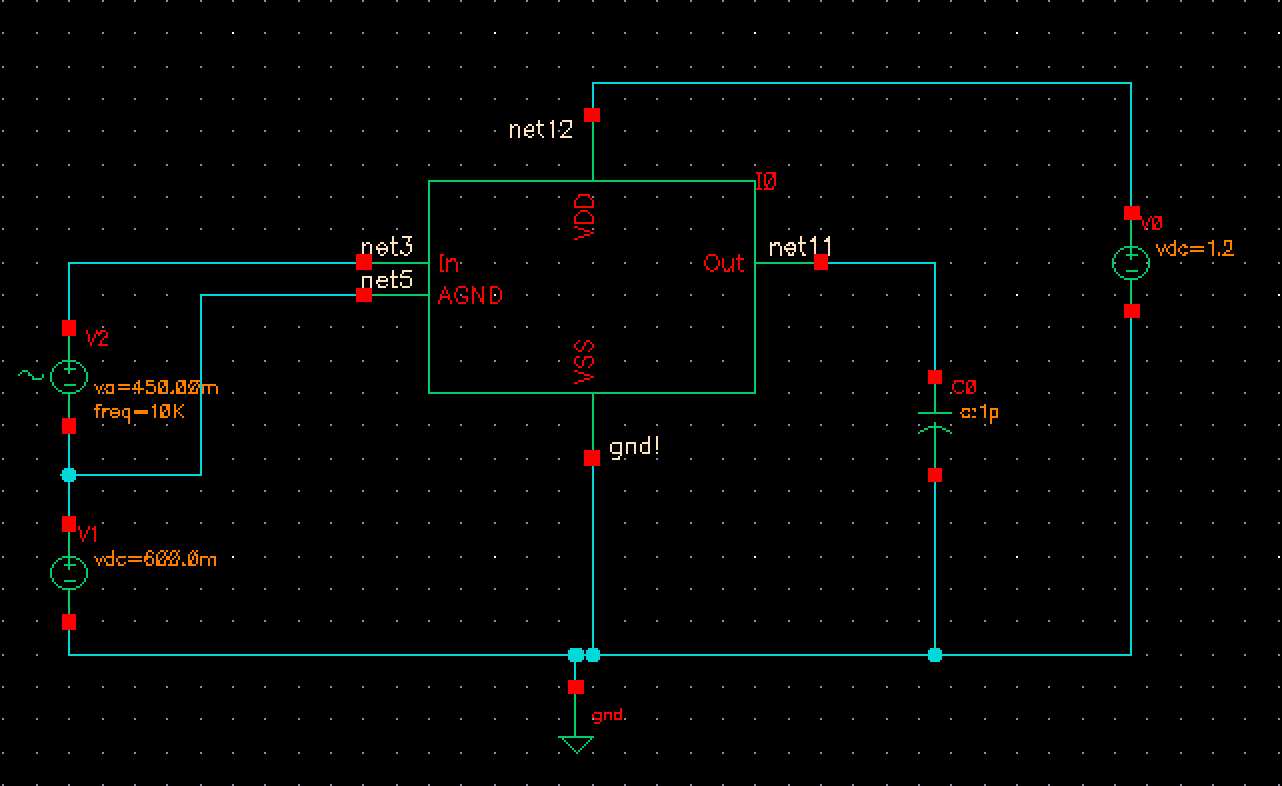
\includegraphics[width=\columnwidth]{schematics/filter_tb.png}
  \caption{A schematic of the test-bench used to measure the AC and transient performance of the filter.}
  \label{fig:filter_tb}
\end{figure}

We first measured the transient performance of the filter by using a $\SI{0.9}{\volt}$ peak-peak, $\SI{10}{\kilo\hertz}$ sine wave centered around $\SI{0.6}{\volt}$ as an input. The resulting input and output are shown in \Cref{fig:filter_tran}. This figure shows that the output signal has no significant distortion even at full range. In fact, we can compute the total harmonic distortion as only $\SI{0.040}{\percent}$, which shows that the circuit meets the voltage swing requirement of the $\Delta \Sigma$ converter.

\begin{figure}[!htb]
  \centering
  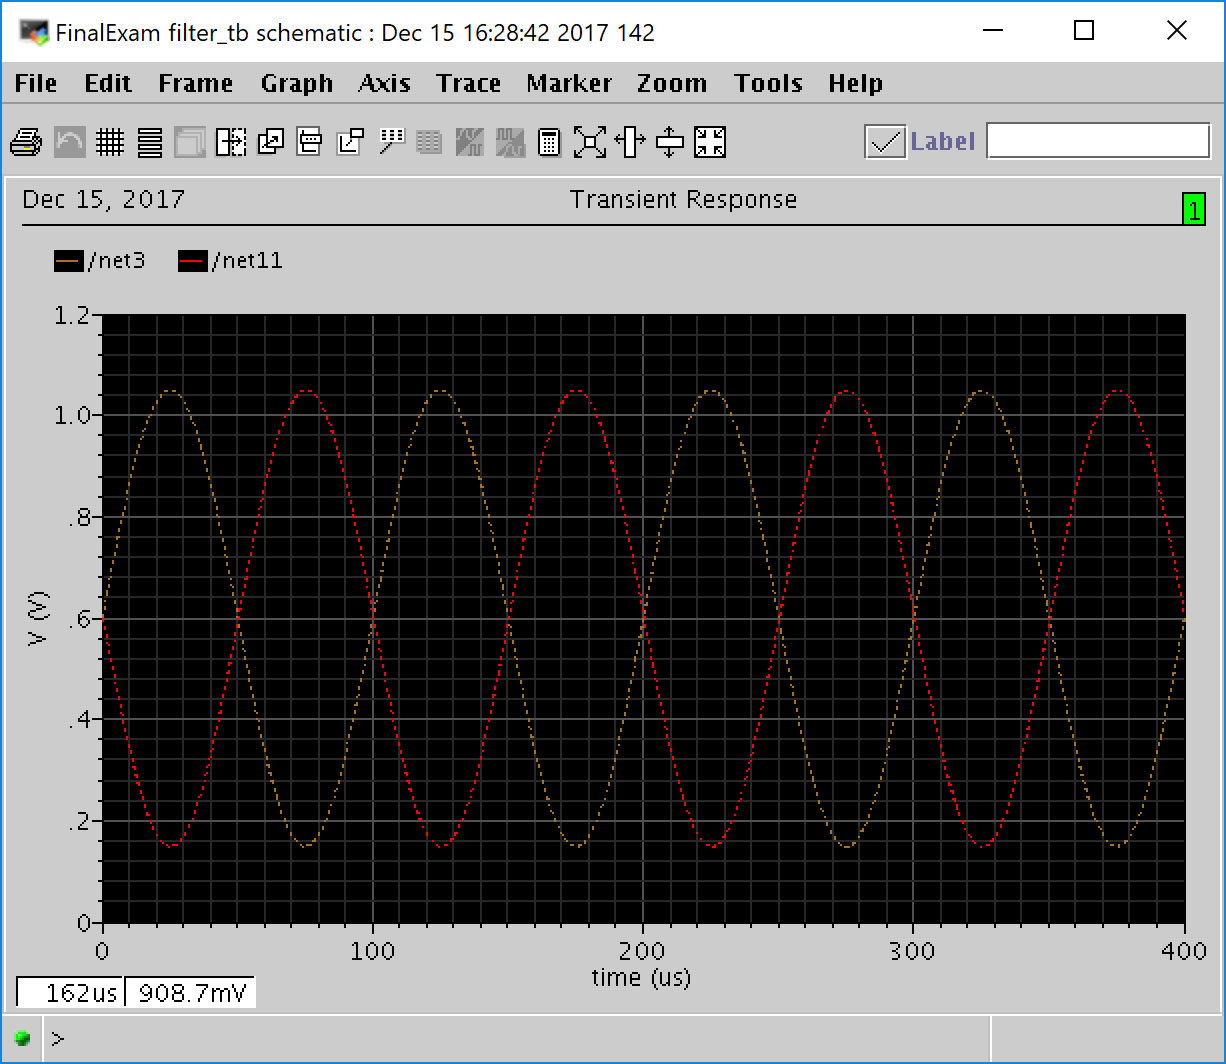
\includegraphics[width=\columnwidth]{results/filter_tran.png}
  \caption{Transient response of the filter for a $\SI{0.9}{\volt}$ peak-peak, $\SI{10}{\kilo\hertz}$ sine wave centered around $\SI{0.6}{\volt}$. The input waveform is shown in brown and the output waveform is shown in red.}
  \label{fig:filter_tran}
\end{figure}

We then measured the AC performance of the filter by using small signal analysis. The results are shown in \Cref{fig:filter_ac}. These results show that we have a DC gain of $\SI{0.99953}{\volt\per\volt}$, an attenuation of $\SI{0.053}{\deci\bel}$ and a phase shift of $\SI{8.83}{\degree}$ at $\SI{100}{\kilo\hertz}$, and an attenuation of $\SI{41.5}{\deci\bel}$ at $\SI{15}{\mega\hertz}$. Therefore, the filter meets all the AC requirements.

\begin{figure}[!htb]
  \centering
  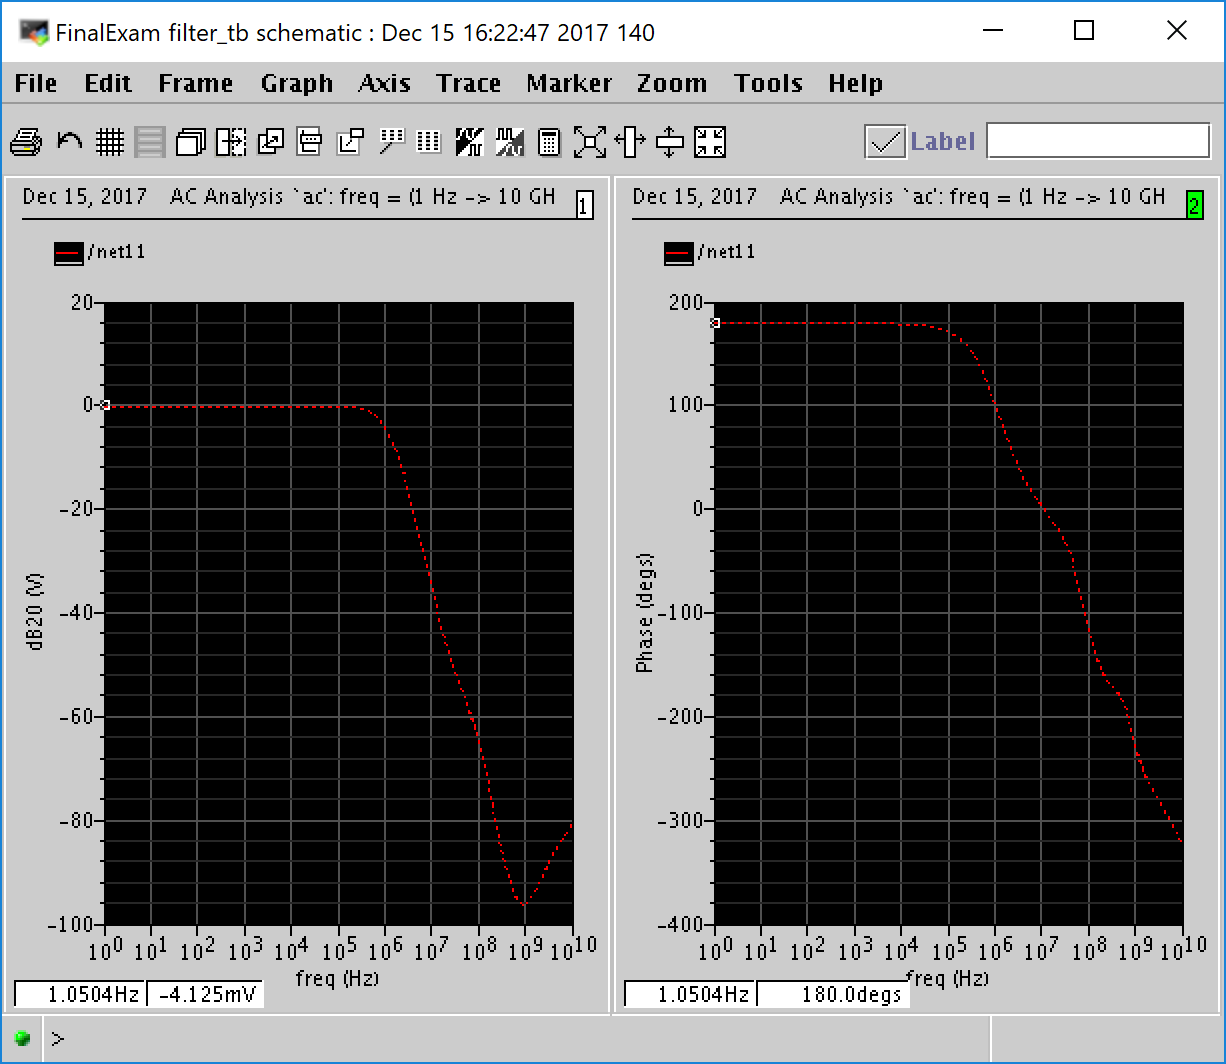
\includegraphics[width=\columnwidth]{results/filter_ac.png}
  \caption{AC response of the filter. The plot on the left shows the gain in $\SI{}{\deci\bel}$ and the plot on the right shows the phase in $\SI{}{\degree}$.}
  \label{fig:filter_ac}
\end{figure}

We next measured the noise properties of the filter. After running an AC noise analysis and integrating the results from $\SI{1}{\hertz}$ to $\SI{100}{\kilo\hertz}$, we obtained the results shown in \Cref{fig:filter_noise}. This figure clearly shows that we have a total RMS output noise of $\SI{66}{\micro\volt}$, which meets the specified maximum noise level for the input to the $\Delta \Sigma$ converter.

\begin{figure}[!htb]
  \centering
  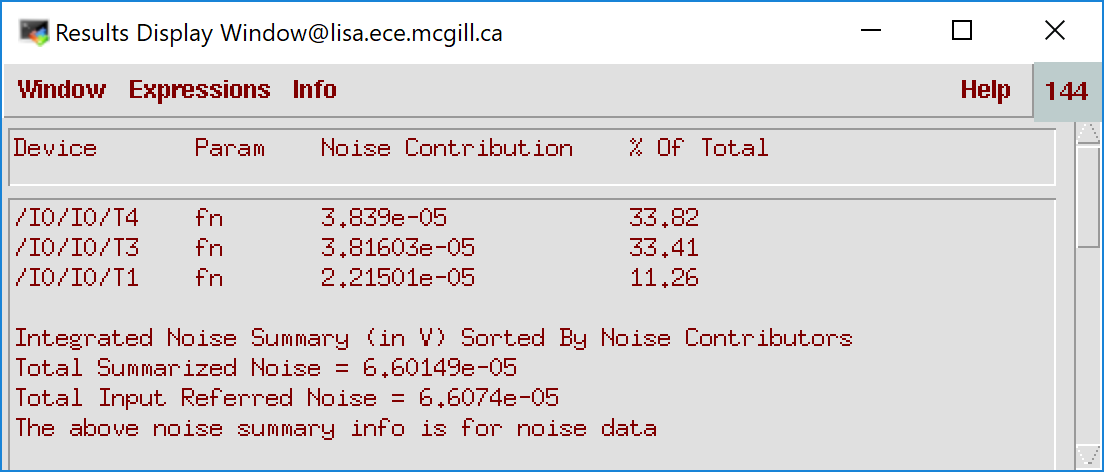
\includegraphics[width=\columnwidth]{results/filter_noise.png}
  \caption{Noise results for the filter over the bandwidth from $\SI{1}{\hertz}$ to $\SI{100}{\kilo\hertz}$.}
  \label{fig:filter_noise}
\end{figure}

Then, we measured the output resistance of the filter using the circuit shown in \Cref{fig:filter_tb_2}. With the load resistance set to $\SI{20}{\ohm}$ and the input set to $\SI{1}{\volt}$, we measured a small signal output voltage of $\SI{0.6984}{\volt}$. Using a simple voltage divider equation, we found that the output resistance of the filter was therefore $\SI{8.62}{\ohm}$, which is smaller than the maximum output resistance requirement.

\begin{figure}[!htb]
  \centering
  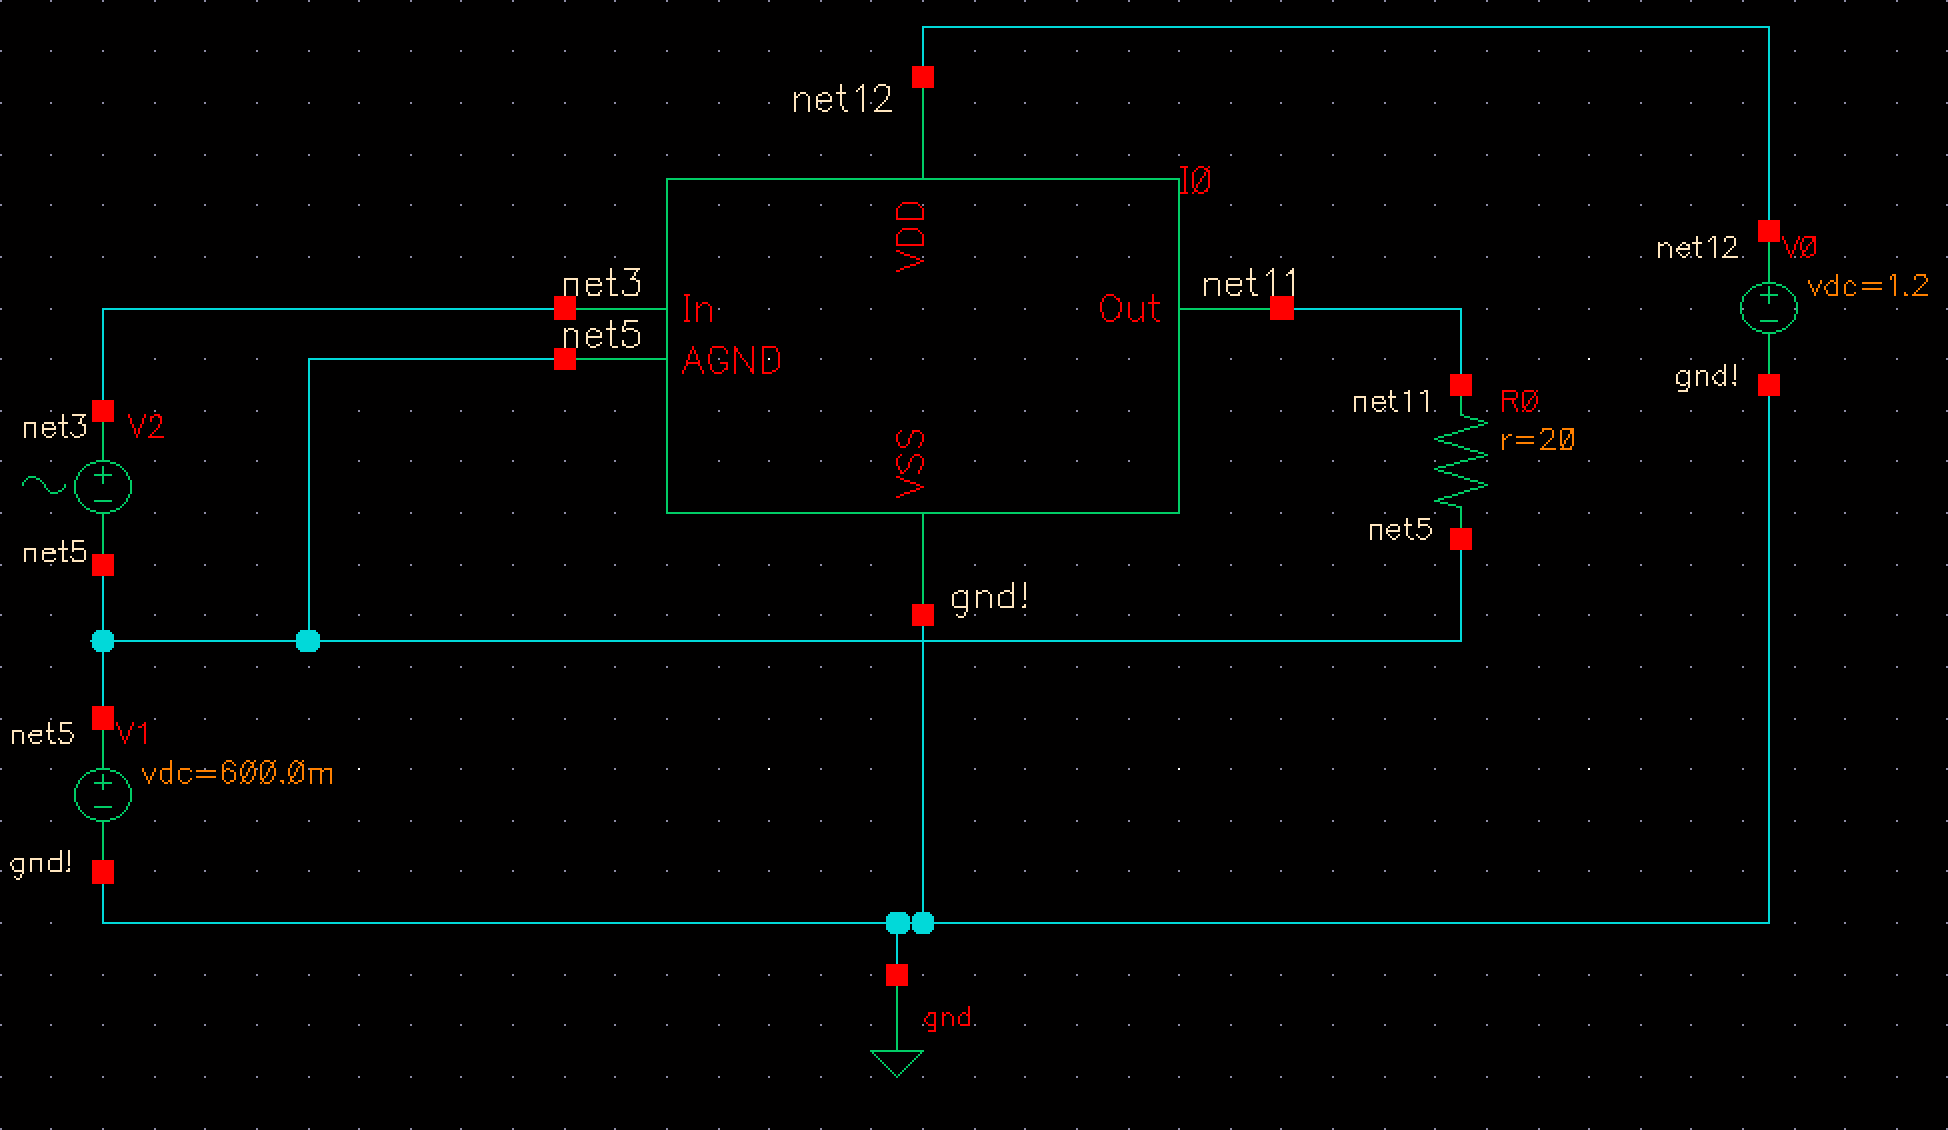
\includegraphics[width=\columnwidth]{schematics/filter_tb_2.png}
  \caption{A schematic of the test-bench used to measure the output resistance of the filter.}
  \label{fig:filter_tb_2}
\end{figure}

Finally, we measured the input resistance of the filter using the circuit shown in \Cref{fig:filter_tb_3}. With the signal resistance set to $\SI{40}{\kilo\ohm}$ and the input set to $\SI{1}{\volt}$, we measured a small signal output voltage of $\SI{0.49962}{\volt}$. Using a simple voltage divider equation, we found that the input resistance of the filter was therefore $\SI{39.98}{\kilo\ohm}$, which greatly exceeds the specification.

\begin{figure}[!htb]
  \centering
  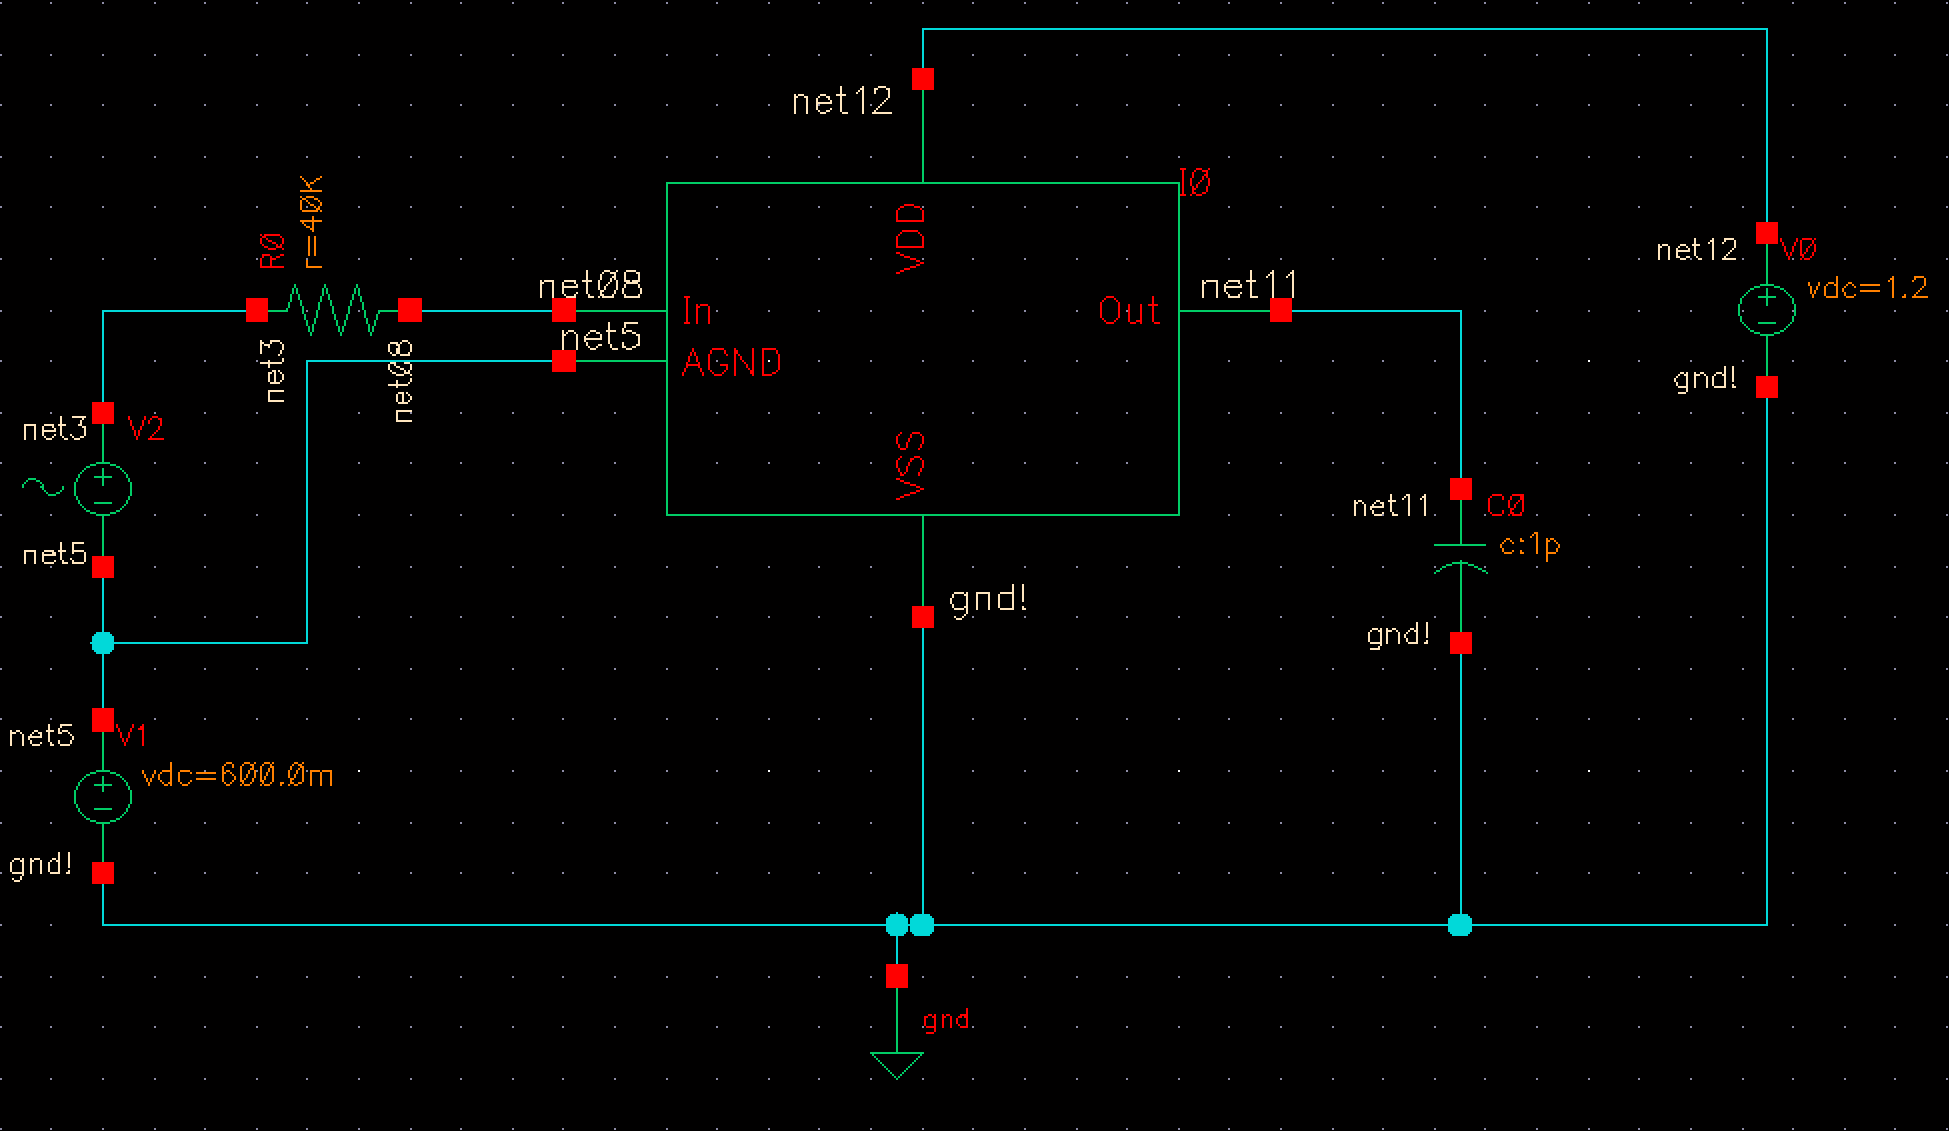
\includegraphics[width=\columnwidth]{schematics/filter_tb_3.png}
  \caption{A schematic of the test-bench used to measure the input resistance of the filter.}
  \label{fig:filter_tb_3}
\end{figure}

\section{Layout}

Next, we planned out a rough sketch of the layout for the filter. As shown in \Cref{fig:folded_cascode_2}, we made all transistors multiples of a unit size, which reduces the error when trying to match them. We used a combination of the number of fingers to increase the length of a transistor and the multiplicity to increase the width of a transistor, thus ensuring that transistors can be made into rectangular shapes that are not too long and not too wide.

In addition, we made sure that all transistors that need to be matched have a multiplicity of at least $2$, which allows us to use a common centroid geometry to eliminate the effect of the first order component of the process gradient in producing matching error. An example of this is shown in \Cref{fig:layout_diff_pair}. In this figure, $T_0$ and $T_1$ are placed such that their centroids coincide. In addition, this figure shows the addition of dummy structures to the boundaries of the pair, which ensures that all transistors have a similar environment and thus creates a better matching. The dummy transistors would typically be connected to $V_{SS}$.

\begin{figure}[!htb]
  \centering
  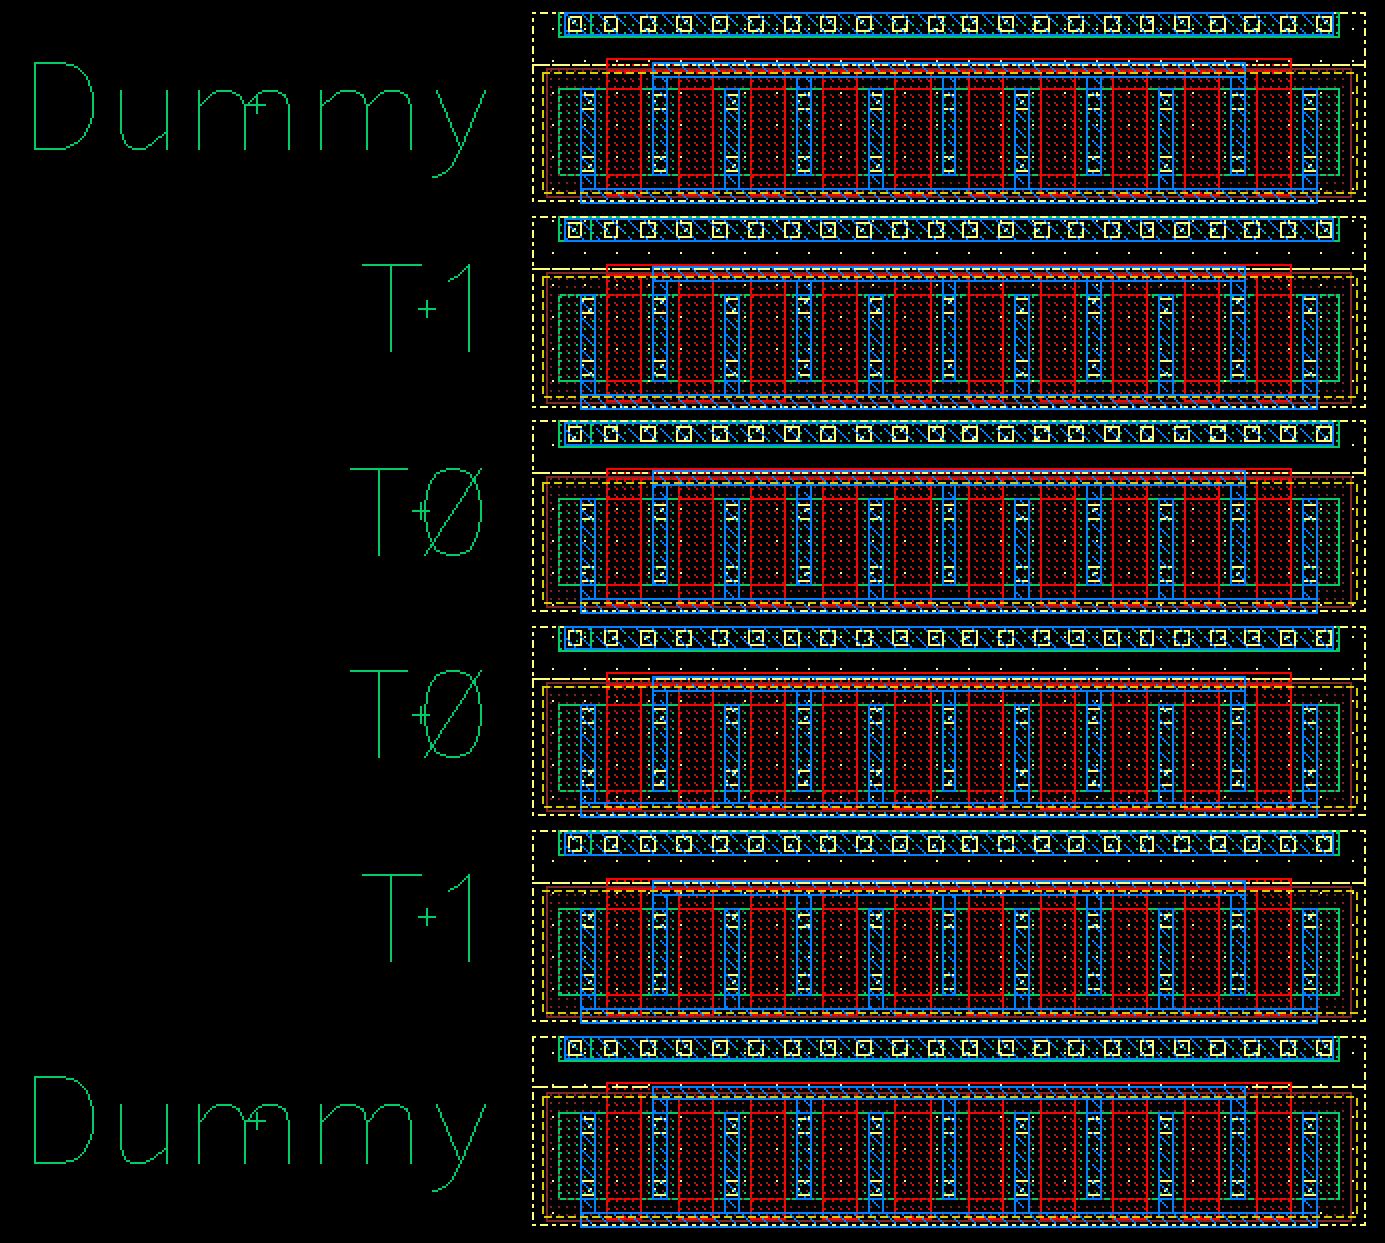
\includegraphics[width=\columnwidth]{layout/diff_pair.png}
  \caption{A common centroid layout for a differential input pair with dummy structures at the boundary. Connections are not shown.}
  \label{fig:layout_diff_pair}
\end{figure}

For the passive components, matching was also critical since it controls the DC gain of the filter. In addition, mismatches can split the poles of the filter, causing ringing to occur. To ensure that these components are matched correctly, we again split them into subcomponents of unit size and used a common centroid geometry. A sketch of the layout of the resistors in the circuit is shown in \Cref{fig:layout_res}, and a sketch of the layout of the capacitors in the circuit is shown in \Cref{fig:layout_cap}.
We note here that while the matching of components is critical, the values of the components themselves are not. Since the $\Delta \Sigma$ converter oversamples at a rate of $\SI{16}{\mega\hertz}$ and the signal bandwidth is only $\SI{100}{\kilo\hertz}$, the resulting pole at around $\SI{1}{\mega\hertz}$ can vary by $\SI{\pm 20}{\percent}$ while still producing little passband attenuation and sufficient stopband attenuation.

\begin{figure}[!htb]
  \centering
  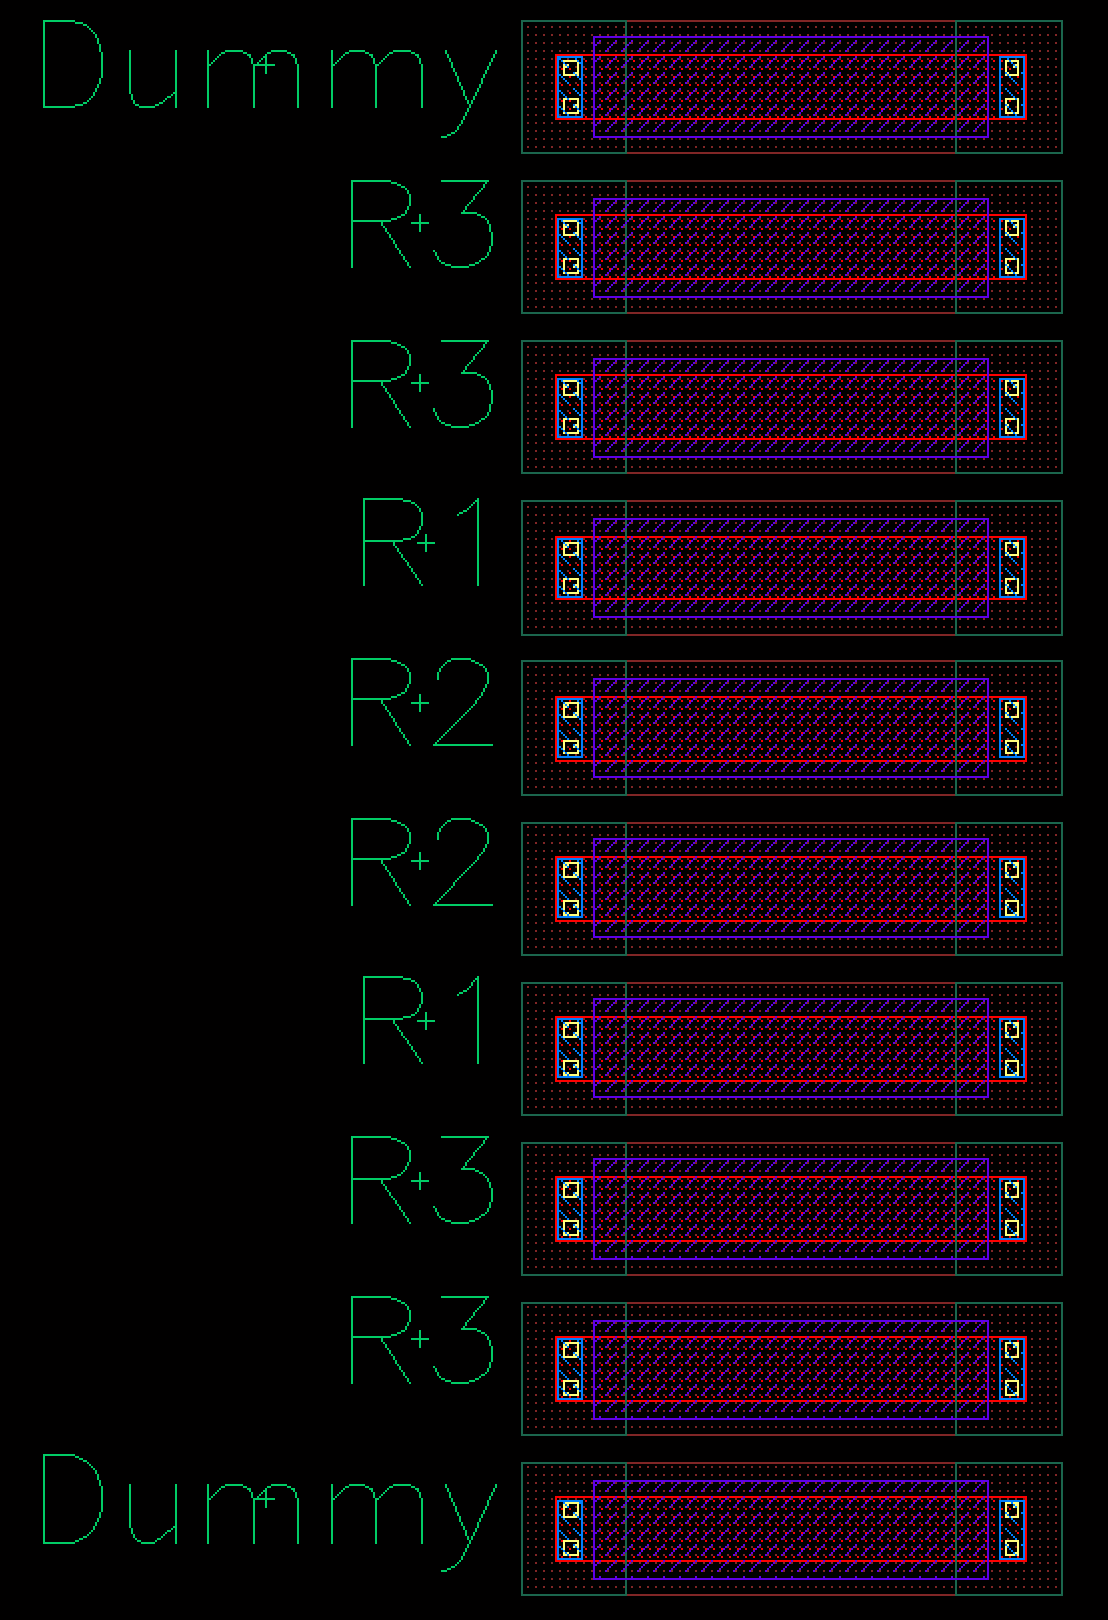
\includegraphics[width=\columnwidth]{layout/res.png}
  \caption{A common centroid layout for the resistors in the filter. Connections are not shown.}
  \label{fig:layout_res}
\end{figure}

\begin{figure}[!htb]
  \centering
  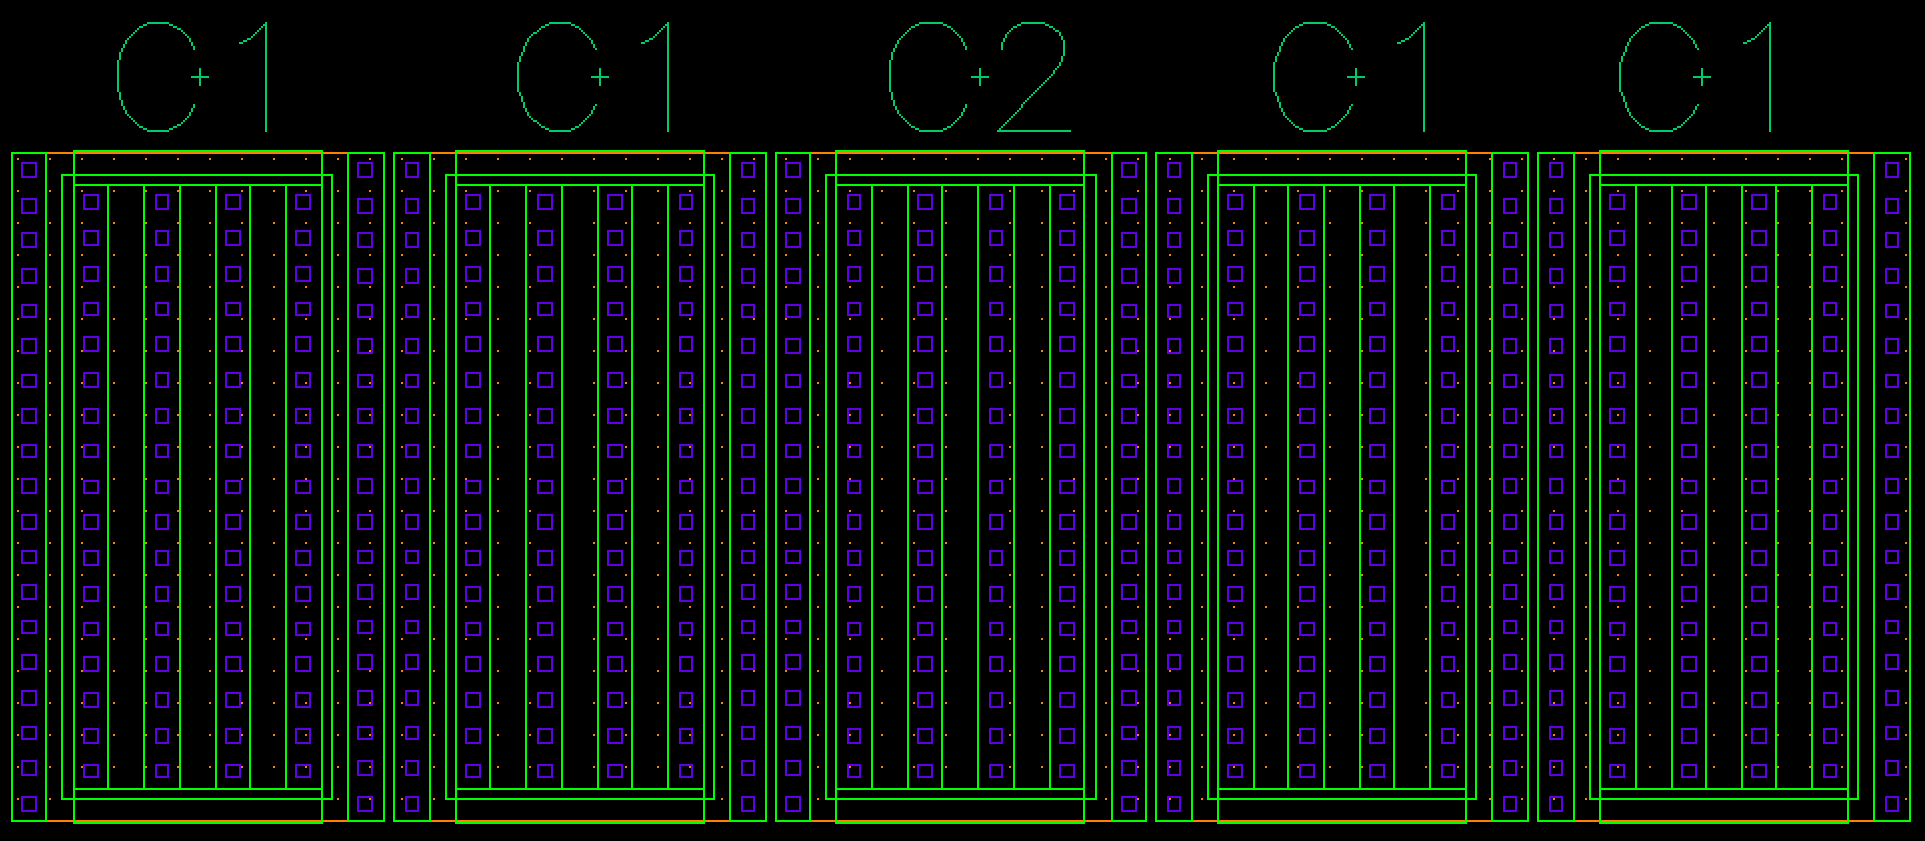
\includegraphics[width=\columnwidth]{layout/cap.png}
  \caption{A common centroid layout for the capacitors in the filter. Connections are not shown.}
  \label{fig:layout_cap}
\end{figure}

\section{Conclusions}

In conclusion, we designed an anti-aliasing filter capable of acting as a preprocessor for the $\Delta \Sigma$ converter specified in the examination question. This filter meets all of the specifications. In addition, we provided a sketch of the approach we would use to lay out such a filter.

\bibliographystyle{IEEEtran}
\bibliography{IEEEabrv,references}

\end{document}
